\section{$\phi$-meson analysis} 
\subsection{Particle reconstruction}
\subsection{Acceptance and efficiency}
\subsubsection{Acceptance}

\begin{figure}[h]
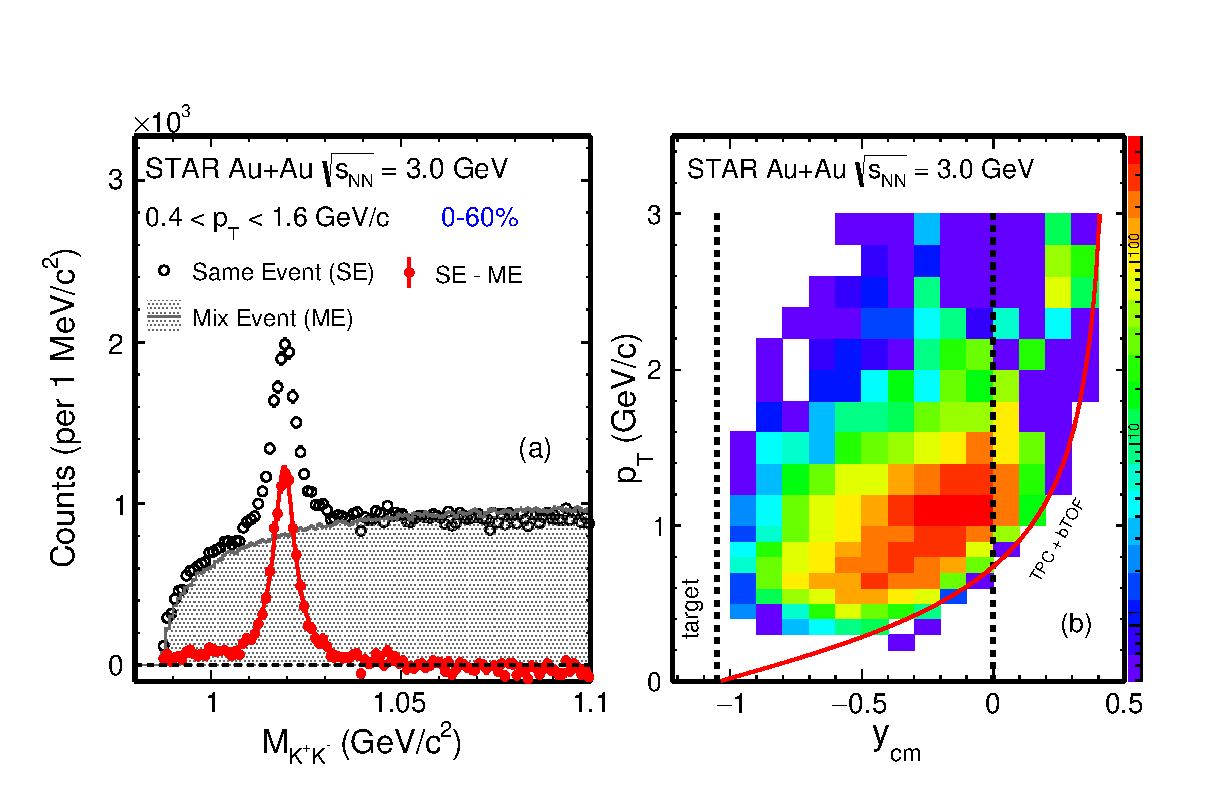
\includegraphics[width=0.85\linewidth]{chapterY/fig/fig1_signal.eps}
  \caption{(a) Invariant mass of $K^+K^-$ pairs in 0-60\% centrality and 0.4--1.6\,GeV/$c$ for the total inclusive yield. (b) The reconstructed $\phi$-meson acceptance $p_T$ vs. rapidity in the center-of-mass frame ($y_{\rm cm}$).}
\label{phiSignal}
\end{figure}

Fig.~\ref{phiSignal} shows the invariant mass of $K^+K^-$ pairs for total inclusive one. Black open circles represent the same-event (SE) unlike-sign (US) distributions. Grey shaded histograms represent the mix-event (ME) US distributions that are used to estimate the combinatorial background. The red solid circles depict the $\phi$-meson signals obtained by subtracting the ME combinatorial background from the SE distributions. (b) The reconstructed $\phi$-meson acceptance $p_T$ vs. rapidity in the center-of-mass frame ($y_{\rm cm}$).


\subsubsection{Efficiency corrections}

\begin{figure}[h]
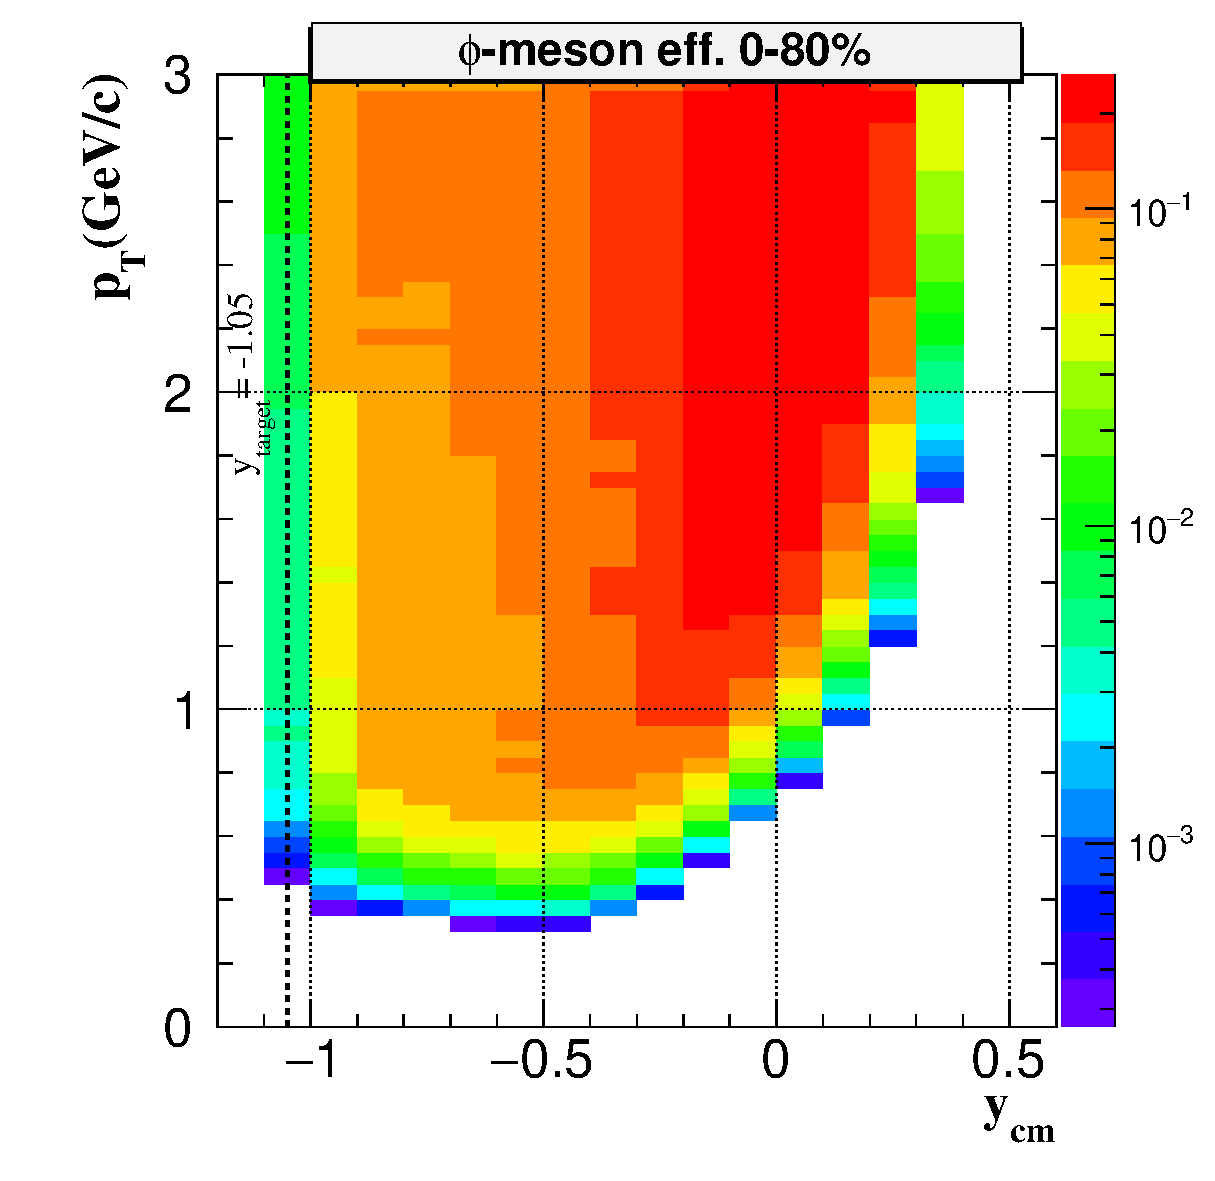
\includegraphics[width=0.6\linewidth]{chapterY/fig/2effAll_rap_0.eps}
\caption{Reconstruction efficiency of $\phi$, as a function of $y$ and $p_{\rm{T}}$ at $\sqrt{s_{NN}}$ = 3 GeV.}
\label{phi_2Deff}
\end{figure}

Fig.~\ref{phi_2Deff} shows the 2D y vs $p_T$ $\phi$-meson reconstruction efficiency of.


\subsection{$v_1$ and $v_2$ extraction}
\subsection{Systematic uncertainties}
\subsubsection{$v_1$}

\begin{figure}[h]
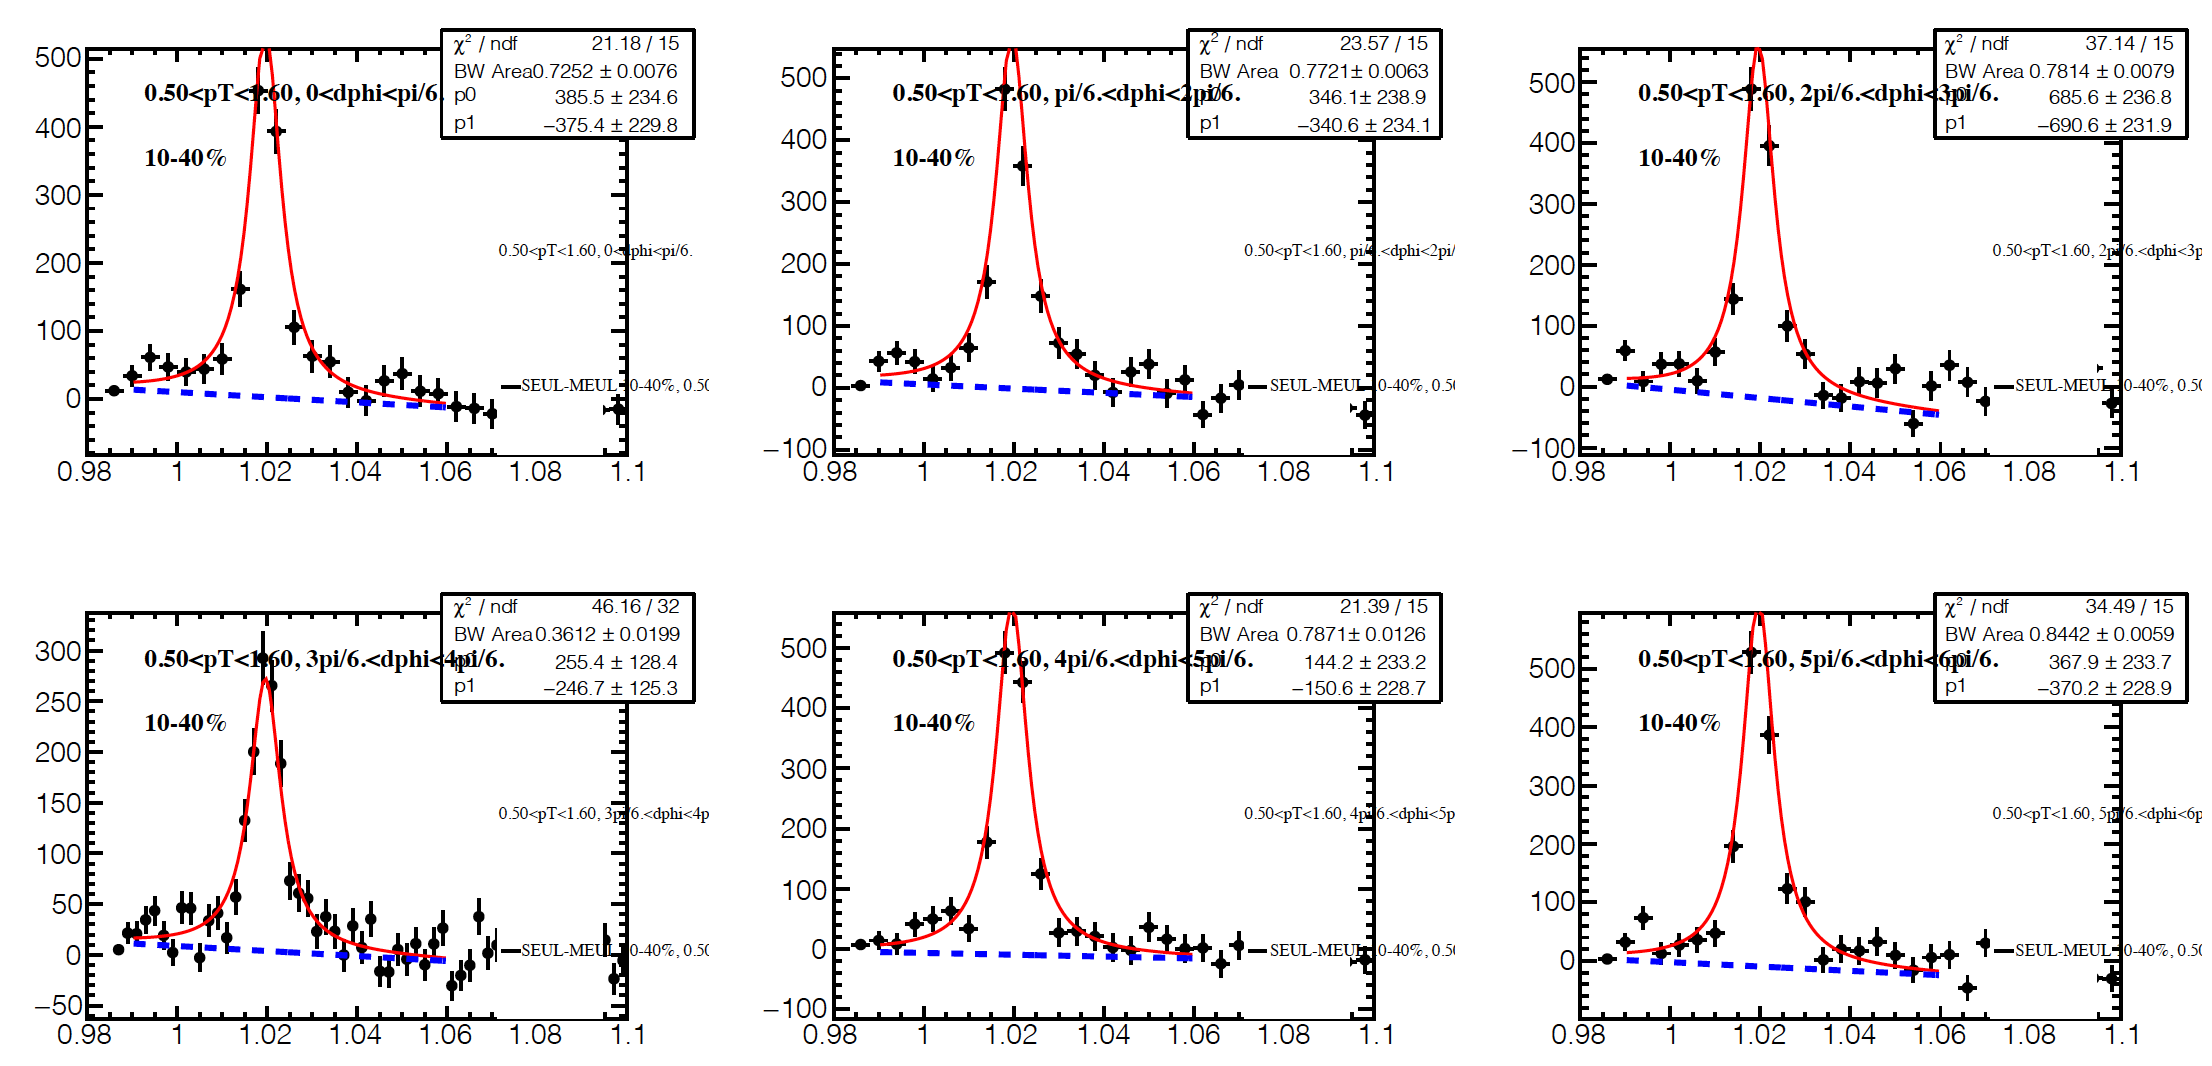
\includegraphics[width=0.85\linewidth]{chapterY/fig/phi_invEP_v1_10_40.png}
\caption{$\phi$-meson signals in several different $\phi$-$\Psi$ range.}
\label{phi_v1}
\end{figure}

\begin{figure}[h]
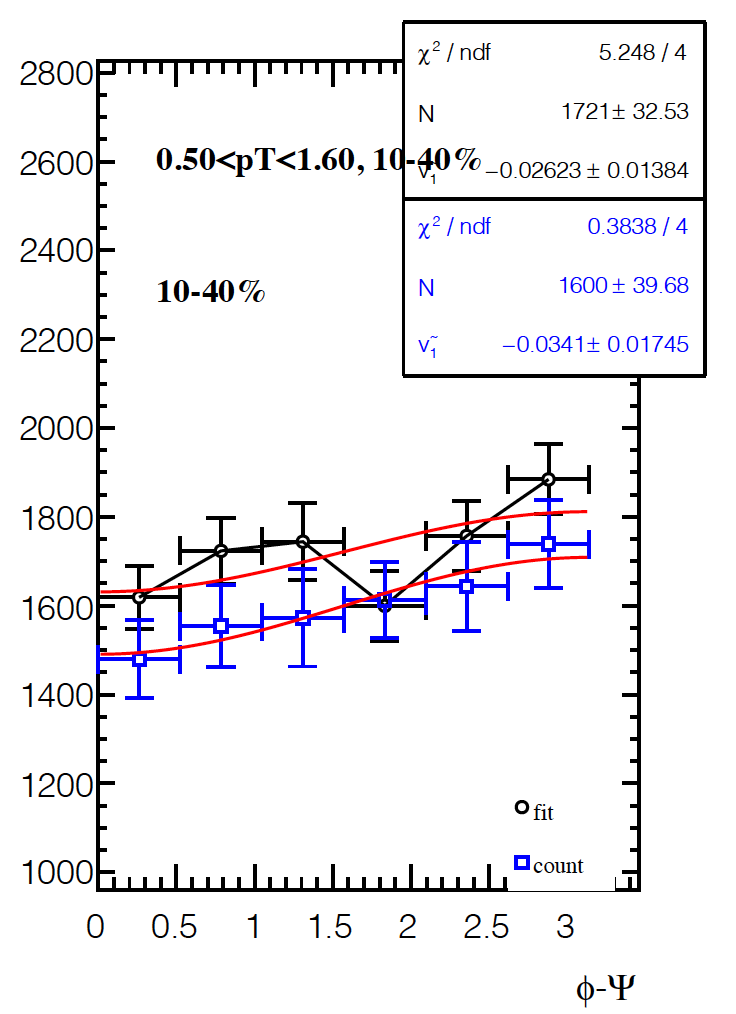
\includegraphics[width=0.6\linewidth]{chapterY/fig/phi_invEP_v1_10_40_fit.png}
  \caption{$\phi$-meson raw counts vs. $\phi$-$\Psi$, fitted with the function to extract the raw v1.}
\label{phi_v1_fit}
\end{figure}

\begin{figure}[h]
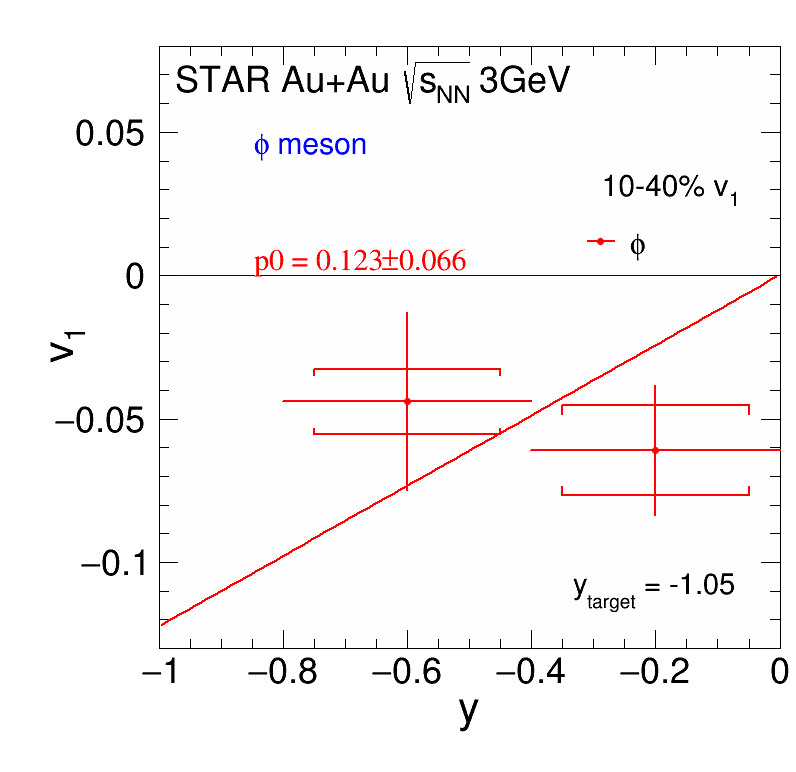
\includegraphics[width=0.49\linewidth]{chapterY/fig/fig1_phi_v1Slop1_10_40.png}
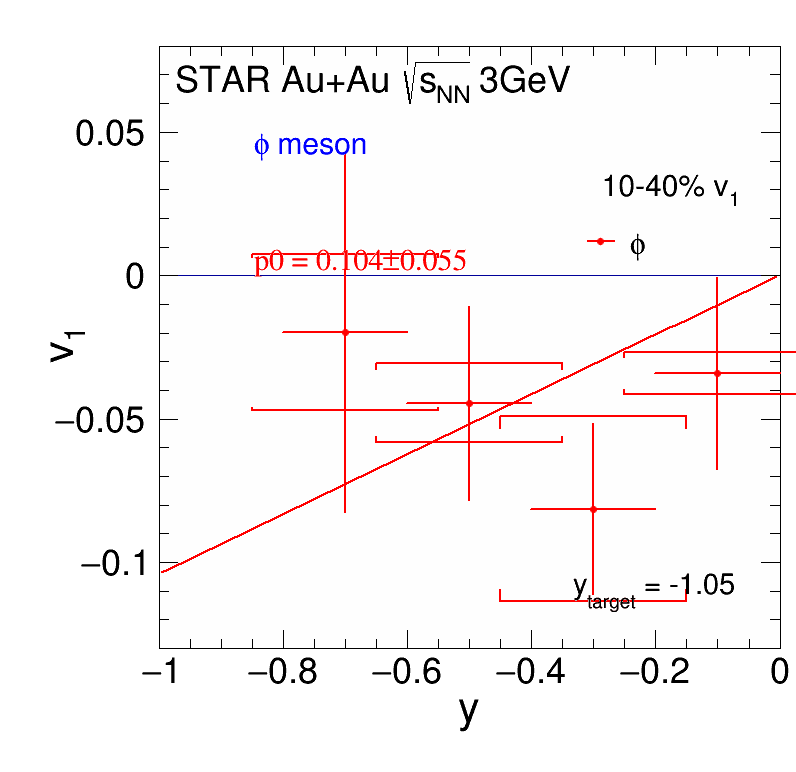
\includegraphics[width=0.49\linewidth]{chapterY/fig/fig1_phi_v1Slop11_10_40.png}
  \caption{$\phi$-meson $v_1$ vs. y, fitted with a linear function cross (0,0).}
\label{phi_dv1dy}
\end{figure}

\subsubsection{$v_2$}

\begin{figure}[h]
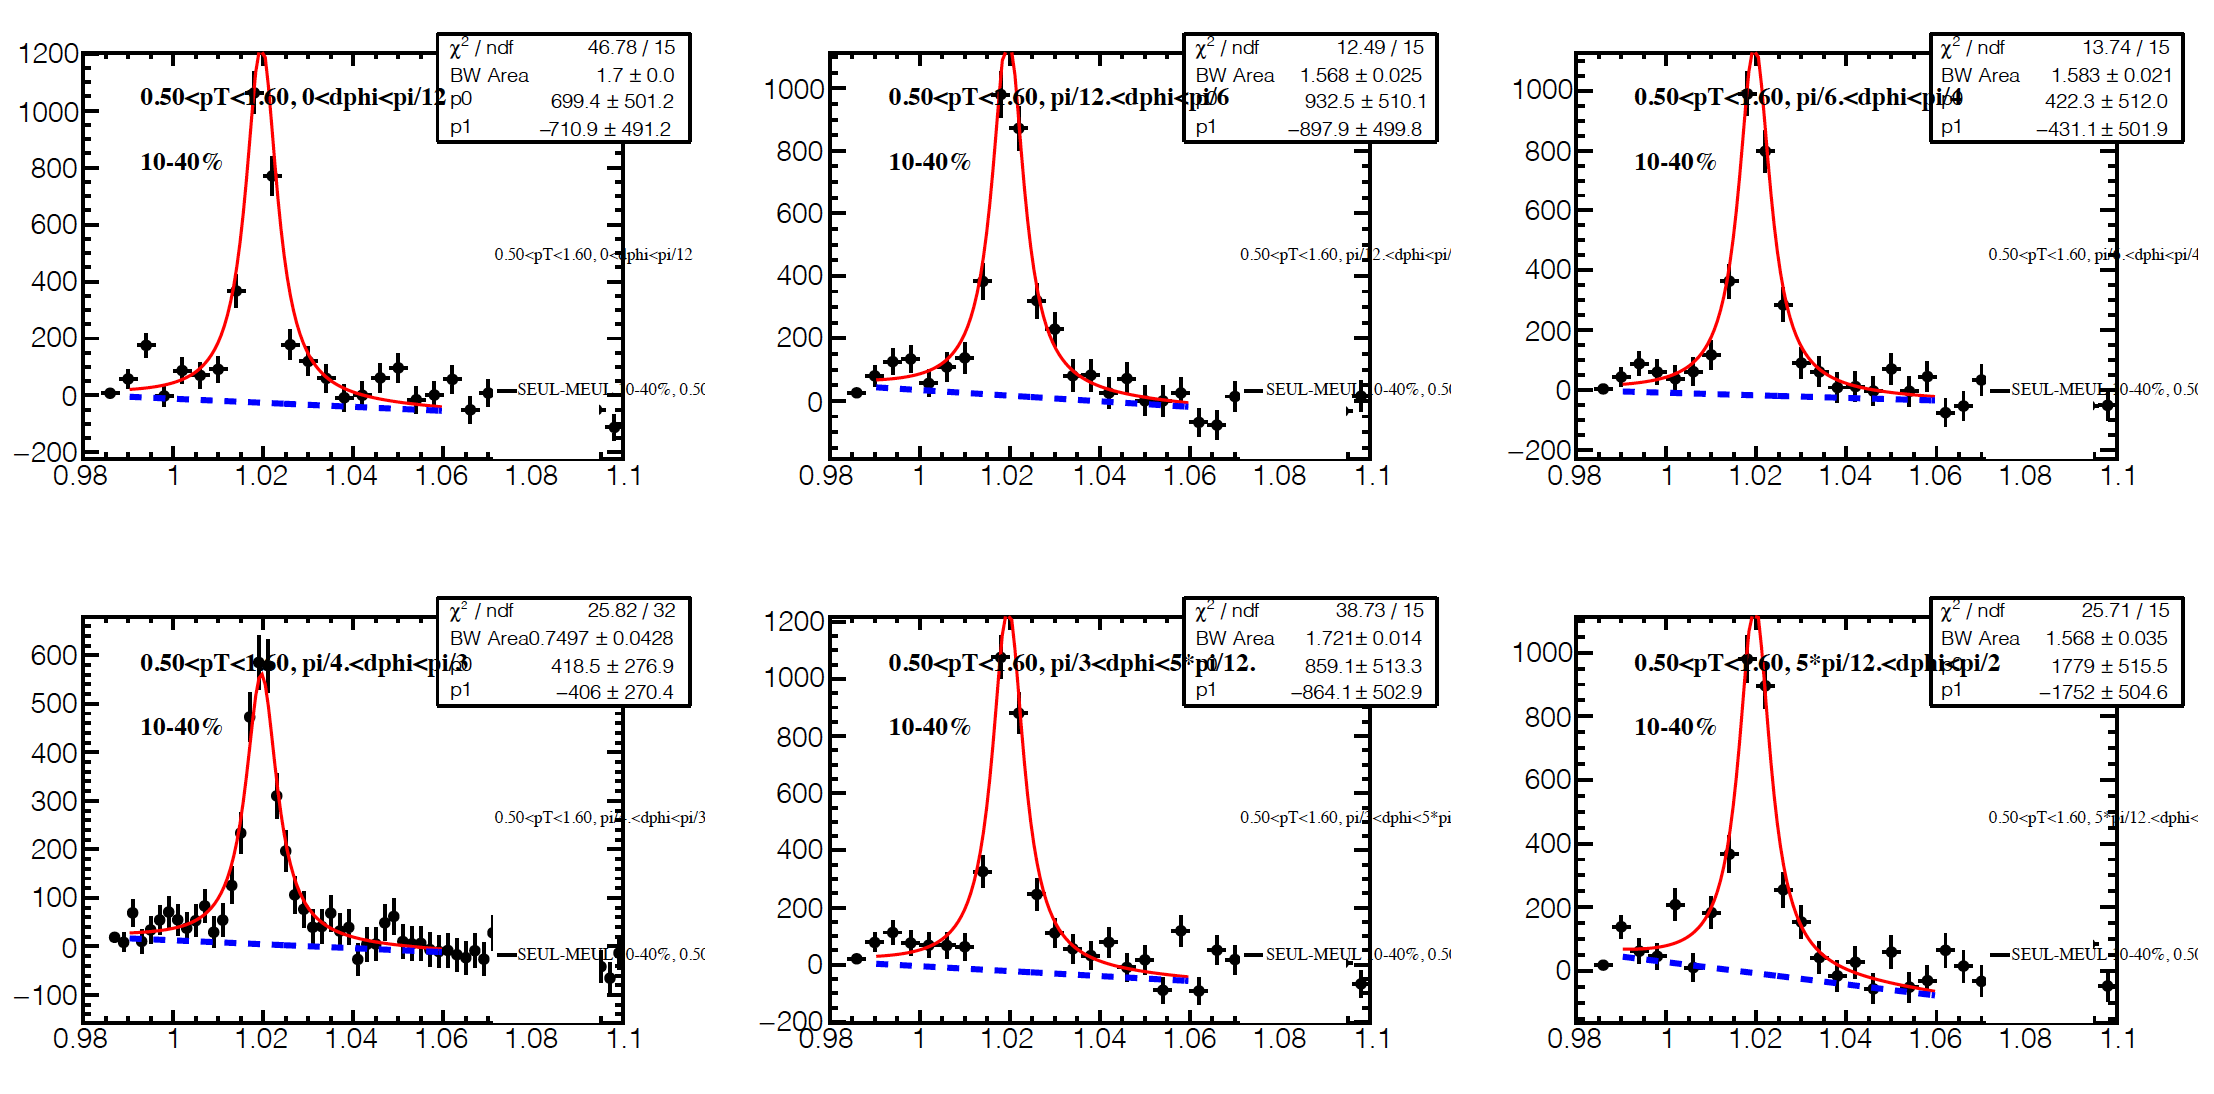
\includegraphics[width=0.85\linewidth]{chapterY/fig/phi_invEP_v2_10_40.png}
\caption{$\phi$-meson signals in several different $\phi$-$\Psi$ range.}
\label{phi_v2}
\end{figure}

\begin{figure}[h]
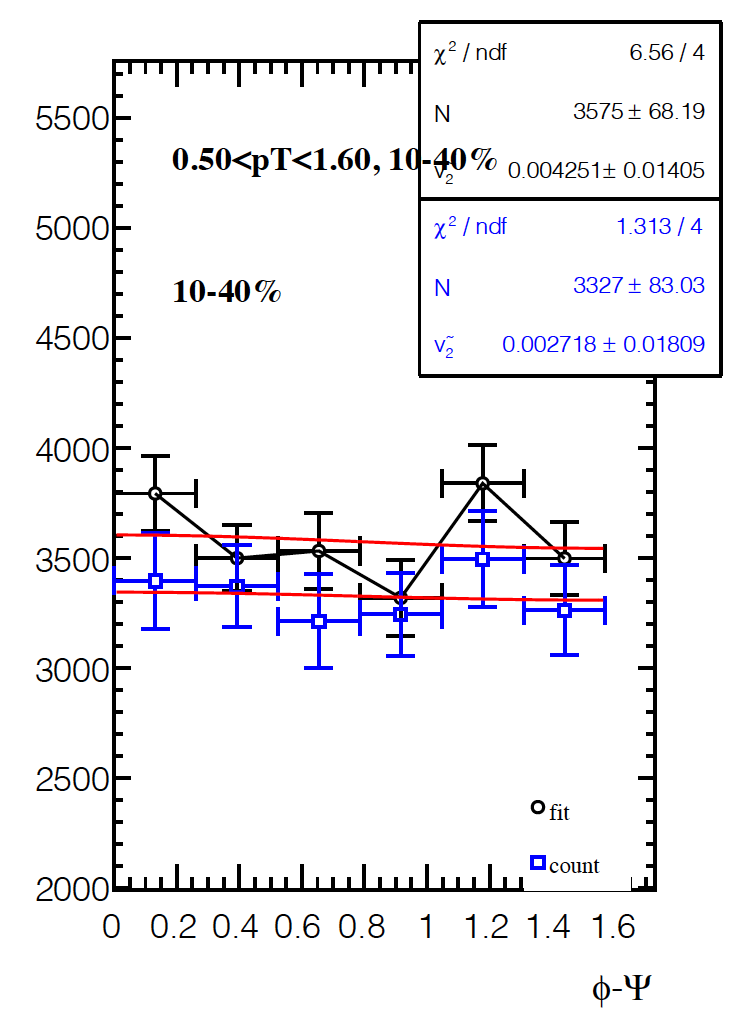
\includegraphics[width=0.6\linewidth]{chapterY/fig/phi_invEP_v2_10_40_fit.png}
\caption{$\phi$-meson raw counts vs. \phi$-$\Psi, fitted with the function to extract the raw v2.}
\label{phi_v2_fit}
\end{figure}

\begin{figure}[h]
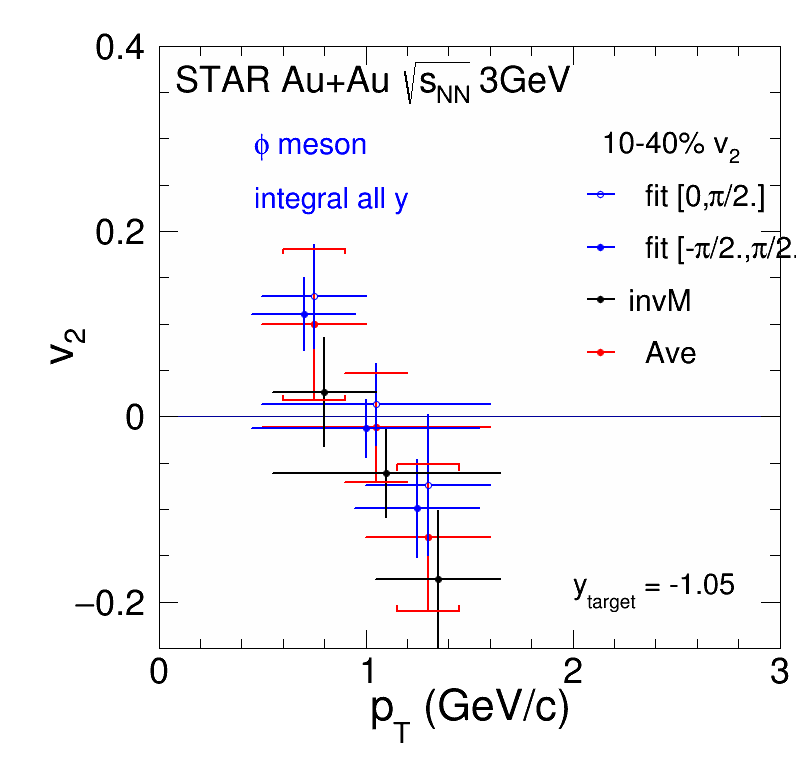
\includegraphics[width=0.49\linewidth]{chapterY/fig/fig1_phi_v2_10_40.png}
  \caption{$\phi$-meson $v_2$ vs. $p_T$, here the three $p_T$ range are from [0.5,1.0],[1.0,1.6],[0.5,1.6].}
\label{phi_v2pT}
\end{figure}

\subsection{Results}
\subsubsection{$v_1$ results for $\phi$-meson}

\begin{figure}[h]
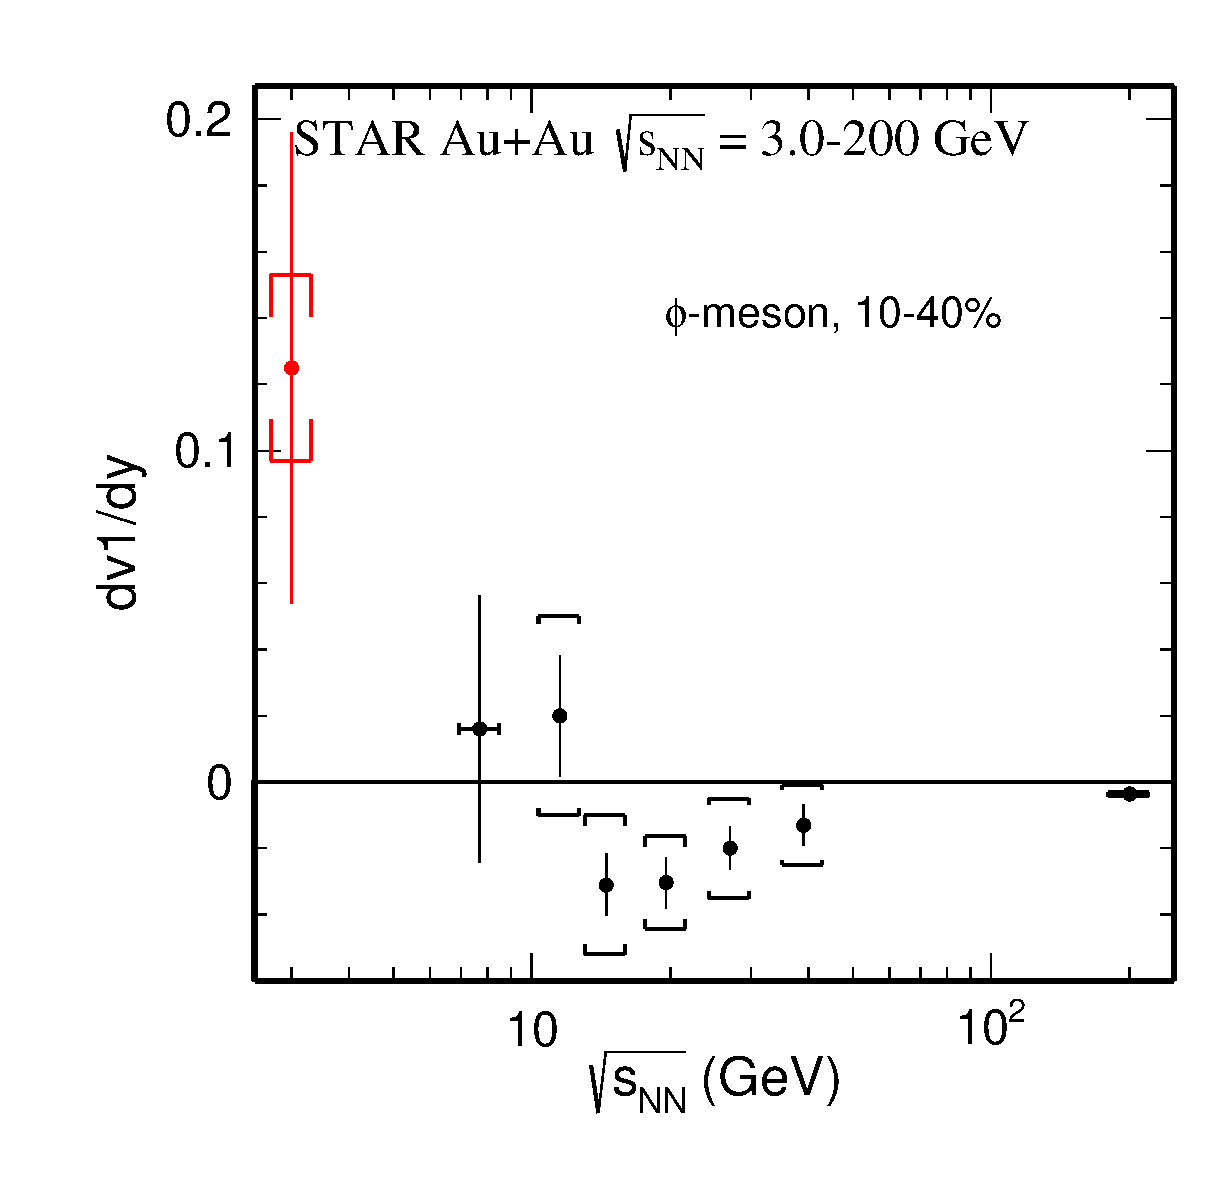
\includegraphics[width=0.6\linewidth]{chapterY/fig/Fffig_dv1_vs_sNN.eps}
\caption{$\phi$-meson d$v_1$/dy slop as a function of collision energies for $10-40\%$ centrality.}
\label{phi_dv1dy_energy}
\end{figure}

\subsubsection{$v_2$ results for $\phi$-meson}

\begin{figure}[h]
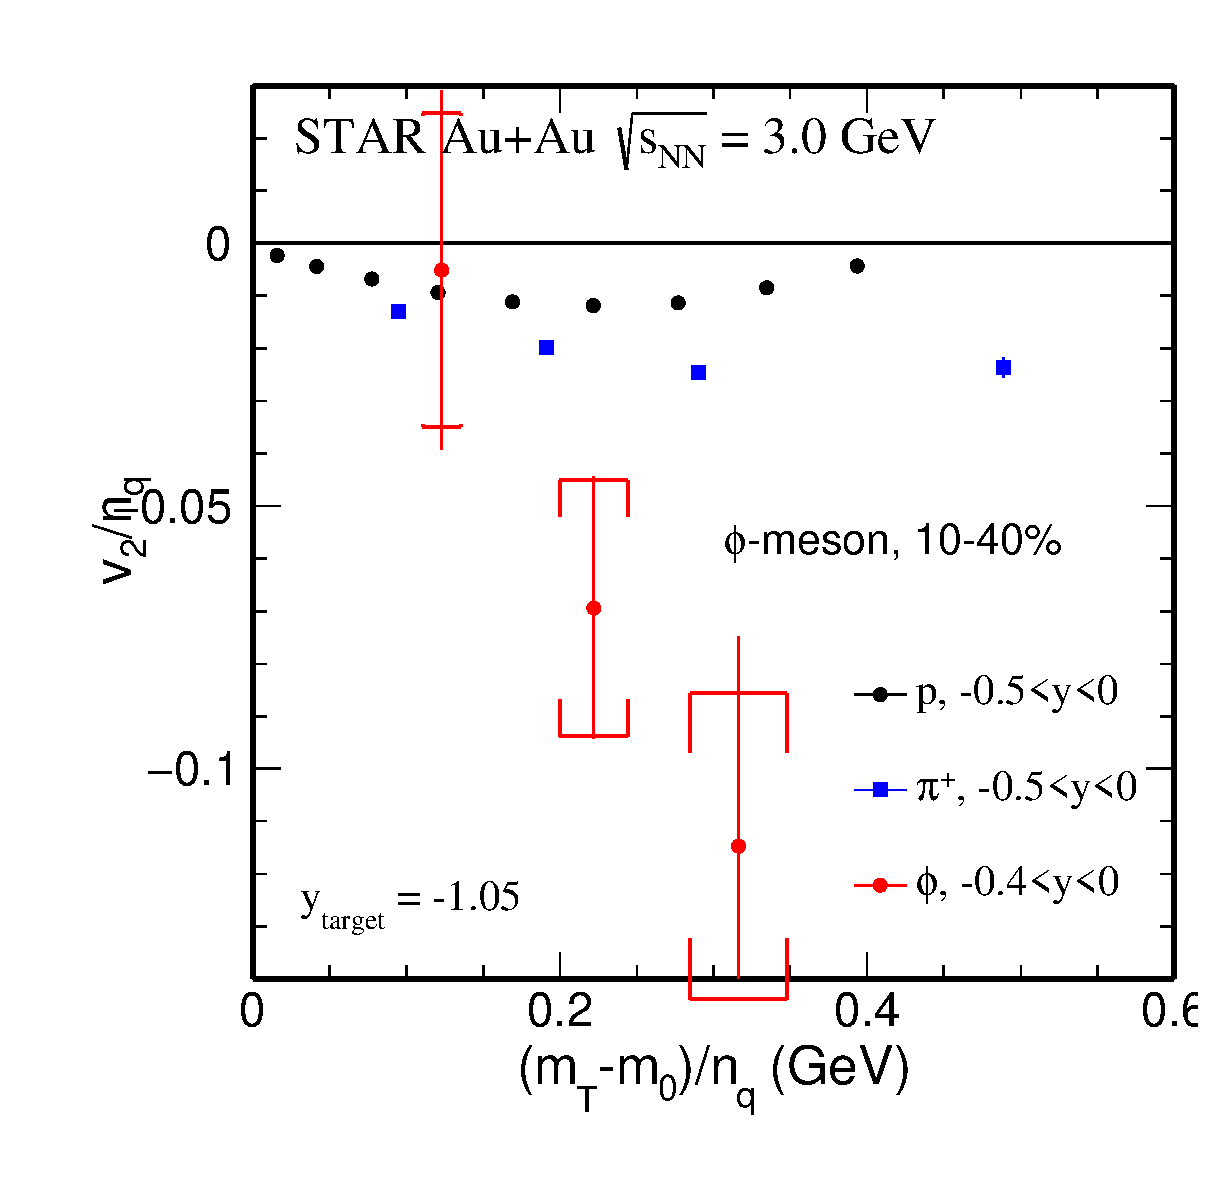
\includegraphics[width=0.6\linewidth]{chapterY/fig/Fffig_v2NCQ_y00p4.eps}
\caption{$\phi$-meson $v_2$/$n_q$ scaling as a function of $m_T-m_0$/$n_q$ for $10-40\%$ centrality and compared with the $\pi$ and p.}
\label{phi_v2_pT}
\end{figure}
